% arch_phase2.tex — Phase 2 (intonation + vibrato; not yet implemented), "architecture-diagram" style (isometric volumes, two branches).
% Standalone TikZ; compile with:  pdflatex arch_phase2.tex
\documentclass[tikz,border=8pt]{standalone}
\usepackage{amsmath,amssymb}
\usepackage[T1]{fontenc}
\usepackage{helvet}
\renewcommand{\familydefault}{\sfdefault}
\usetikzlibrary{positioning,arrows.meta,calc,fit,backgrounds}

% ---- Okabe--Ito, colourblind-safe (as in the reference) ----
\definecolor{gblue}{HTML}{0072B2}   % graph / structure branch
\definecolor{gamber}{HTML}{E69F00}  % evidence / feature branch
\definecolor{ggreen}{HTML}{009E73}  % fusion
\definecolor{gpink}{HTML}{CC79A7}   % inference head
\definecolor{gverm}{HTML}{D55E00}   % likelihood -- the changing part
\definecolor{gink}{HTML}{333333}
\definecolor{ggray}{HTML}{9A9A9A}
\definecolor{ggrey}{HTML}{777777}
\definecolor{gline}{HTML}{555555}
\definecolor{amberink}{HTML}{8A5D00}
\definecolor{pinkink}{HTML}{8E3F6E}
\definecolor{greenink}{HTML}{00795A}

% ---- isometric cuboid:  \cuboid{x}{y}{w}{h}{depth}{colour}{name} ----
\newcommand{\cuboid}[7]{%
  \begin{scope}[shift={(#1,#2)}]
    \fill[#6!45, draw=#6, line width=0.5pt] (0,0) rectangle (#3,#4);
    \fill[#6!22, draw=#6, line width=0.5pt] (0,#4) -- (#5,#4+#5) -- (#3+#5,#4+#5) -- (#3,#4) -- cycle;
    \fill[#6!65, draw=#6, line width=0.5pt] (#3,0) -- (#3+#5,#5) -- (#3+#5,#4+#5) -- (#3,#4) -- cycle;
    \coordinate (#7w) at (0,{#4/2});
    \coordinate (#7e) at ({#3+#5},{#4/2+#5/2});
    \coordinate (#7c) at ({#3/2},{#4/2});
    \coordinate (#7s) at ({#3/2},0);
    \coordinate (#7n) at ({#3/2+#5},{#4+#5});
  \end{scope}}

\begin{document}
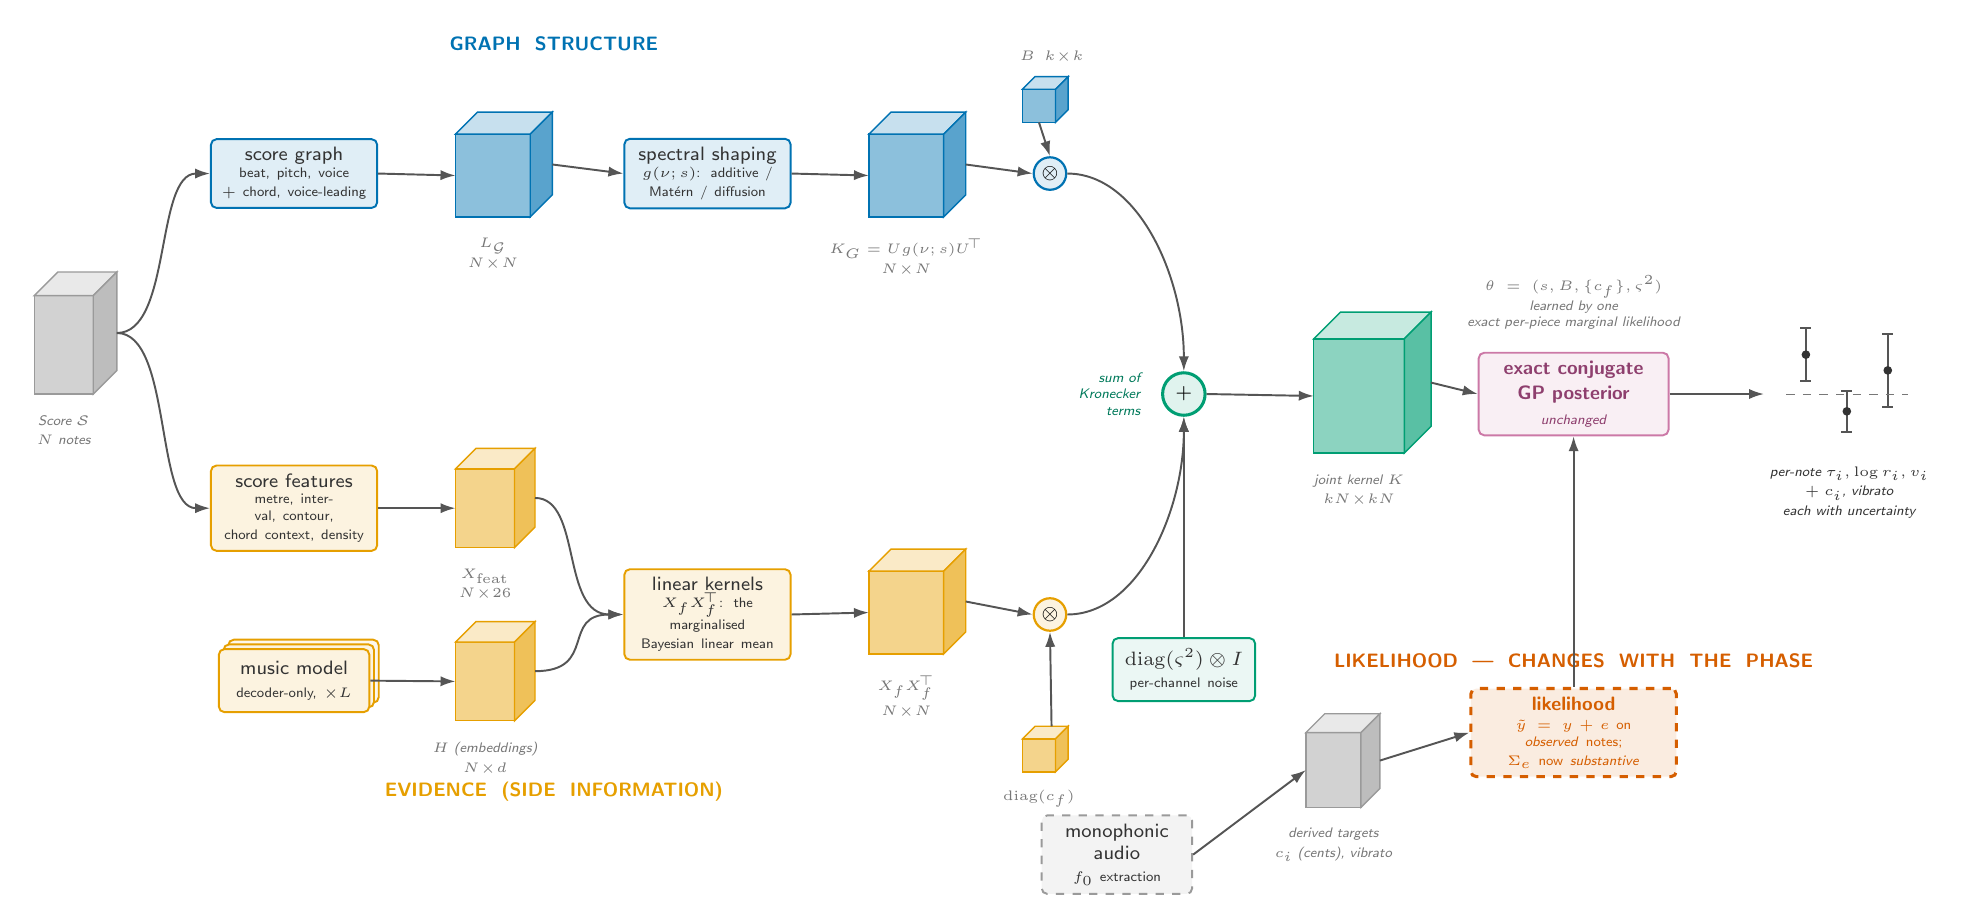
\begin{tikzpicture}[
  font=\scriptsize,
  op/.style   = {rounded corners=2pt, draw=#1, fill=#1!12, line width=0.7pt,
                 align=center, inner sep=3pt, minimum height=8mm, text=gink},
  op/.default = gink,
  arr/.style  = {-{Latex[length=1.9mm,width=1.3mm]}, draw=gline, line width=0.7pt},
  dim/.style  = {font=\tiny\itshape, text=ggrey, align=center},
  sec/.style  = {font=\scriptsize\bfseries, text=#1},
  sec/.default= gink,
]

% ================= INPUT =================
\cuboid{0.0}{-0.1}{0.75}{1.25}{0.30}{ggray}{sc}
\node[dim, below=1.5mm of scs] {Score $\mathcal{S}$\\[1pt] $N$ notes};

% ================= TOP BRANCH : GRAPH STRUCTURE =================
\node[sec=gblue] at (6.6,4.35) {GRAPH\ \ STRUCTURE};

\node[op=gblue, text width=19mm] (gop) at (3.3,2.7) {score graph\\ \tiny beat, pitch, voice\\[-1pt] \tiny $+$ chord, voice-leading};
\cuboid{5.35}{2.15}{0.95}{1.05}{0.28}{gblue}{lg}
\node[dim, below=1.5mm of lgs] {$L_{\mathcal G}$\\[1pt] $N\!\times\!N$};

\node[op=gblue, text width=19mm] (sop) at (8.55,2.7) {spectral shaping\\ \tiny $g(\nu;s)$: additive /\\[-1pt] \tiny Mat\'ern / diffusion};
\cuboid{10.6}{2.15}{0.95}{1.05}{0.28}{gblue}{kg}
\node[dim, below=1.5mm of kgs] {$K_G=U g(\nu;s) U^{\!\top}$\\[1pt] $N\!\times\!N$};

% ================= BOTTOM BRANCH : EVIDENCE =================
\node[sec=gamber] at (6.6,-5.15) {EVIDENCE\ \ (SIDE\ \ INFORMATION)};

\node[op=gamber, text width=19mm] (fop) at (3.3,-1.55) {score features\\ \tiny metre, interval, contour,\\[-1pt] \tiny chord context, density};
\cuboid{5.35}{-2.05}{0.75}{1.0}{0.26}{gamber}{xf}
\node[dim, below=1.5mm of xfs] {$X_{\mathrm{feat}}$\\[1pt] $N\!\times\!26$};

% music model: stacked blocks = xL
\node[op=gamber, text width=17mm, fill=gamber!8] (mm3) at (3.42,-3.62) {};
\node[op=gamber, text width=17mm, fill=gamber!12] (mm2) at (3.36,-3.68) {};
\node[op=gamber, text width=17mm] (mm1) at (3.30,-3.74) {music model\\ \tiny decoder-only, $\times L$};
\cuboid{5.35}{-4.25}{0.75}{1.0}{0.26}{gamber}{hh}
\node[dim, below=1.5mm of hhs] {$H$ (embeddings)\\[1pt] $N\!\times\!d$};

\node[op=gamber, text width=19mm] (lin) at (8.55,-2.9) {linear kernels\\ \tiny $X_f X_f^{\!\top}$: the marginalised\\[-1pt] \tiny Bayesian linear mean};
\cuboid{10.6}{-3.4}{0.95}{1.05}{0.28}{gamber}{xx}
\node[dim, below=1.5mm of xxs] {$X_f X_f^{\!\top}$\\[1pt] $N\!\times\!N$};

% ================= KRONECKER LIFTS =================
\cuboid{12.55}{3.35}{0.42}{0.42}{0.16}{gblue}{bb}
\node[dim, above=0.5mm of bbn] {$B$\ \ $k\!\times\!k$};
\node[circle, draw=gblue, fill=gblue!12, line width=0.8pt, inner sep=1.3pt] (kron1) at (12.9,2.7) {$\otimes$};

\cuboid{12.55}{-4.9}{0.42}{0.42}{0.16}{gamber}{cc}
\node[dim, below=1.0mm of ccs] {$\operatorname{diag}(c_f)$};
\node[circle, draw=gamber, fill=gamber!12, line width=0.8pt, inner sep=1.3pt] (kron2) at (12.9,-2.9) {$\otimes$};

% ================= FUSION =================
\node[circle, draw=ggreen, fill=ggreen!12, line width=1.1pt, inner sep=2.6pt] (plus) at (14.6,-0.1) {$+$};
\node[dim, text=greenink, left=1.4mm of plus, align=right] {sum of\\ Kronecker\\ terms};
\node[op=ggreen, text width=16mm, fill=ggreen!8] (noise) at (14.6,-3.6) {$\operatorname{diag}(\varsigma^2)\otimes I$\\ \tiny per-channel noise};

\cuboid{16.25}{-0.85}{1.15}{1.45}{0.34}{ggreen}{kk}
\node[dim, below=1.5mm of kks] {joint kernel $K$\\[1pt] $kN\!\times\!kN$};

% ================= HEAD =================
\node[op=gpink, text width=22mm, text=pinkink] (head) at (19.55,-0.1)
  {\textbf{exact conjugate}\\[1pt] \textbf{GP posterior}\\[1pt] \tiny\itshape unchanged};
\node[dim, above=1.6mm of head, text width=30mm]
  {$\theta=(s,B,\{c_f\},\varsigma^2)$ learned by one\\ exact per-piece marginal likelihood};

% ================= LIKELIHOOD (the changing part) =================
\node[op=ggray, text width=17mm, dashed] (aud) at (13.75,-5.95) {monophonic audio\\ \tiny $f_0$ extraction};
\cuboid{16.15}{-5.35}{0.7}{0.95}{0.24}{ggray}{ob}
\node[dim, below=1.4mm of obs] {derived targets\\[1pt] $c_i$ (cents), vibrato};

\node[op=gverm, text width=24mm, line width=1.1pt, text=gverm, dashed] (lik) at (19.55,-4.4)
  {\textbf{likelihood}\\[1pt] \tiny $\tilde y=y+e$ on \emph{observed} notes;\\[-1pt] \tiny $\Sigma_e$ now \emph{substantive}};
\node[sec=gverm, above=1.2mm of lik] {LIKELIHOOD\ \ ---\ \ CHANGES\ \ WITH\ \ THE\ \ PHASE};

% ================= OUTPUT : estimates with error bars =================
\begin{scope}[shift={(22.5,-0.1)}]
  \foreach \x/\v/\e in {0/0.50/0.34, 0.52/-0.22/0.26, 1.04/0.30/0.46} {
    \draw[gline, line width=0.7pt] (\x,{\v-\e}) -- (\x,{\v+\e});
    \draw[gline, line width=0.7pt] ({\x-0.07},{\v-\e}) -- ({\x+0.07},{\v-\e});
    \draw[gline, line width=0.7pt] ({\x-0.07},{\v+\e}) -- ({\x+0.07},{\v+\e});
    \fill[gink] (\x,\v) circle (0.055);
  }
  \draw[ggrey, line width=0.3pt, dashed] (-0.25,0) -- (1.30,0);
\end{scope}
\node[dim, text=gink] at (23.05,-1.35)
  {per-note $\tau_i,\log r_i,v_i$\\[1pt] $+\ c_i$, vibrato\\[1pt] each with uncertainty};

% ================= ARROWS =================
\draw[arr] (sce) .. controls +(0.7,0) and +(-0.7,0) .. (gop.west);
\draw[arr] (sce) .. controls +(0.7,0) and +(-0.7,0) .. (fop.west);
\draw[arr] (gop.east) -- (lgw);
\draw[arr] (lge) -- (sop.west);
\draw[arr] (sop.east) -- (kgw);
\draw[arr] (fop.east) -- (xfw);
\draw[arr] (mm1.east) -- (hhw);
\draw[arr] (hhe) .. controls +(0.8,0) and +(-0.8,0) .. (lin.west);
\draw[arr] (xfe) .. controls +(0.6,0) and +(-0.8,0) .. (lin.west);
\draw[arr] (lin.east) -- (xxw);
\draw[arr] (kge) -- (kron1.west);
\draw[arr] (bbs) -- (kron1.north);
\draw[arr] (xxe) -- (kron2.west);
\draw[arr] (ccn) -- (kron2.south);
\draw[arr] (kron1.east) .. controls +(0.9,0) and +(0,1.2) .. (plus.north);
\draw[arr] (kron2.east) .. controls +(0.9,0) and +(0,-1.2) .. (plus.south);
\draw[arr] (noise.north) -- (plus.south);
\draw[arr] (plus.east) -- (kkw);
\draw[arr] (kke) -- (head.west);
\draw[arr] (aud.east) -- (obw);
\draw[arr] (obe) -- (lik.west);
\draw[arr] (lik.north) -- (head.south);
\draw[arr] (head.east) -- ++(1.2,0);

\end{tikzpicture}
\end{document}
